\documentclass[border=2pt]{standalone}
%
\usepackage{amsmath}
\usepackage{siunitx}
\usepackage{wasysym}
\usepackage{empheq}
\usepackage[most]{tcolorbox}
%
%
\usepackage{tikz}
%


\renewcommand{\vec}[1]{\boldsymbol{#1}}  % math vector

\newtcbox{\mymath}[1][]{%
    nobeforeafter, math upper, tcbox raise base,
    enhanced, colframe=blue!30!black,
    colback=blue!30, boxrule=1pt,
    #1}

%\begin{empheq}[box={\mymath[colback=red!30,drop lifted shadow, sharp corners]}]{equation*}
%    c_i = \langle\psi|\phi\rangle
%\end{empheq}

% \psset{unit=1cm} it is a default dimension 1cm

\begin{document}
	
	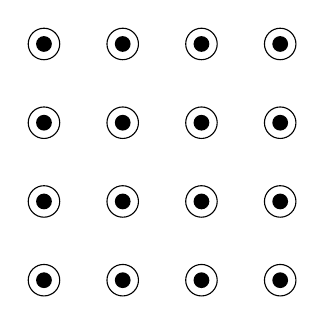
\begin{tikzpicture}
		\foreach \x in {0,1,2,3}
		\foreach \y in {0,1,2,3}
		{
			\draw (\x,\y) circle (0.2cm);
			\fill (\x,\y) circle (0.1cm);
		}
	\end{tikzpicture}

	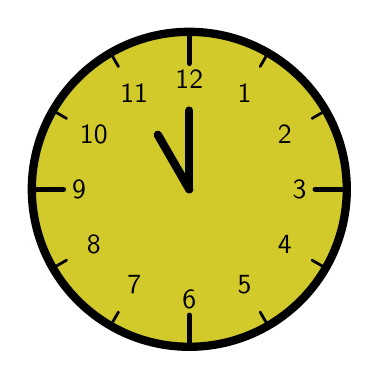
\begin{tikzpicture}[line cap=round,line width=3pt]
		\filldraw [fill=yellow!80!black] (0,0) circle (2cm);

		\foreach \angle / \label in
		{0/3, 30/2, 60/1, 90/12, 120/11, 150/10, 180/9,
		210/8, 240/7, 270/6, 300/5, 330/4}
		{
			\draw[line width=1pt] (\angle:1.8cm) -- (\angle:2cm);
			\draw (\angle:1.4cm) node{\textsf{\label}};
		}

		\foreach \angle in {0,90,180,270}
			\draw[line width=2pt] (\angle:1.6cm) -- (\angle:2cm);

		\draw (0,0) -- (120:0.8cm); % hour
		\draw (0,0) -- (90:1cm);    % minute
	\end{tikzpicture}
	
\end{document}

